\documentclass[fleqn]{article}
\usepackage[spanish,es-noshorthands]{babel}
\usepackage[utf8]{inputenc} 
\usepackage[papersize={5.5in,8.5in},left=1cm, right=1cm, top=1.5cm, bottom=1.7cm]{geometry}
\usepackage{mathexam}
\usepackage{amsmath}
\usepackage{graphicx}
\usepackage{multicol}
\ExamClass{
\includegraphics[height=16pt]{Images/logo-sed.png} Matemáticas $9^{\circ}$}
\ExamName{``Números racionales''}
\ExamHead{
\includegraphics[height=16pt]{Images/logo-colegio.png} IEDAB}
\newcommand{\LineaNombre}{%
\par
\vspace{\baselineskip}
Nombre:\hrulefill \; Curso: \underline{\hspace*{48pt}} \; Fecha: \underline{\hspace*{2.5cm}} \relax
\par}
\let\ds\displaystyle

\begin{document}
\ExamInstrBox{
Respuesta sin justificar mediante procedimiento no será tenida en cuenta en la calificación. Escriba sus respuestas en el espacio indicado. Tiene 45 minutos para contestar esta prueba.}
\LineaNombre
\begin{enumerate}
 \item Calcule ordenadamente
 \begin{enumerate}
 \item $5+2\cdot 3-7\cdot (-1)$\noanswer[.2in]
 \item $8\div (-4)-6\cdot (-3)-80\div 5 =$\noanswer[.2in]
   \item $-32\div \{3-[7-12-(9-5)]+14\}=$\noanswer[.2in]
 \item $2^{2}\cdot 3\cdot 5-2\cdot (-1)+7\cdot (-2)^{3}+(-3)\cdot (-7)=$\noanswer[.2in]
 \end{enumerate}
 \item Calcule el M.C.D. y el m.c.m. de 24, 36 y 72 \noanswer[.75in]
 \item Dadas las siguientes fracciones: $\dfrac{45}{36}$, $\dfrac{90}{180}$, $\dfrac{500}{400}$, $\dfrac{108}{288}$, $\dfrac{80}{64}$, $\dfrac{96}{192}$, $\dfrac{125}{100}$, $\dfrac{105}{280}$
 \begin{enumerate}
 \item Halla la fracción irreducible de cada una de ellas.
 \item Agrupa las que sean equivalentes.
 \item Ordena de menor a mayor los representantes canónicos obtenidos.
 \end{enumerate}
 \noanswer
  \newpage
 \item Efectúe ordenadamente las siguientes operaciones:
 \begin{enumerate}
 \item $\dfrac{1}{2}-\dfrac{1}{4}\cdot \dfrac{1}{8}-\dfrac{1}{16}=$\noanswer[.5in]
 \item $\left(\dfrac{3}{5}-\dfrac{1}{4}+2\right)-\left(\dfrac{3}{4}-\dfrac{2}{5}+1\right)=$\noanswer[.5in]
 \end{enumerate}
 \item De las siguientes figuras, ¿qué fracción representa la parte sombreada de cada una de ellas?
 \begin{enumerate}
 \begin{multicols}{2}
 \item  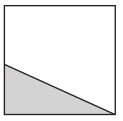
\includegraphics[scale=.8]{Images/Pantallazo-46.png}
 \item 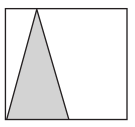
\includegraphics[scale=.8]{Images/Pantallazo-47.png} 
 \end{multicols}
 \end{enumerate}
 \item Calcule la diagonal de una cancha de voleibol de 18 m de largo por 9 metros de ancho.\noanswer

 \end{enumerate}

\end{document}
